\chapter{Results}

This section describes the results from the previously defined experiments.
Similar to the experiments section these results are separated into two
categories being microbenchmarks and applications.

For each result we explain the information being presented as well as further
findings. In addition, probably causes are discussed as well as
potential future experiments to investigate these claims.

\section{Microbenchmarks}

Several of the results for microbenchmarks are grouped together such as
sequential read and write results. Furthermore, all microbenchmark results use
line-graphs scaled with $log4$ on the horizontal axis. Using this scaling the
distance between different file and request sizes is proportional to their
difference in size.

\subsection{Sequential Results}

Our first results compare the sequential read and write performance of F2FS
against FluffleFS. These results are shown in figures
\ref{figure:readsequential} and \ref{figure:writesequential} respectively.
While the performance is similar for the smallest 64KiB file size each larger
filesize constitutes and increasingly larger performance gap. Notable
observations include the large difference between the minimum and
maximum write throughput in F2FS as well as a collapse in throughput for files
beyond 256MiB in size. A similar but much smaller drop can also be observed in
write throughput for FluffleFS.

\begin{figure}[h]
    \centering
	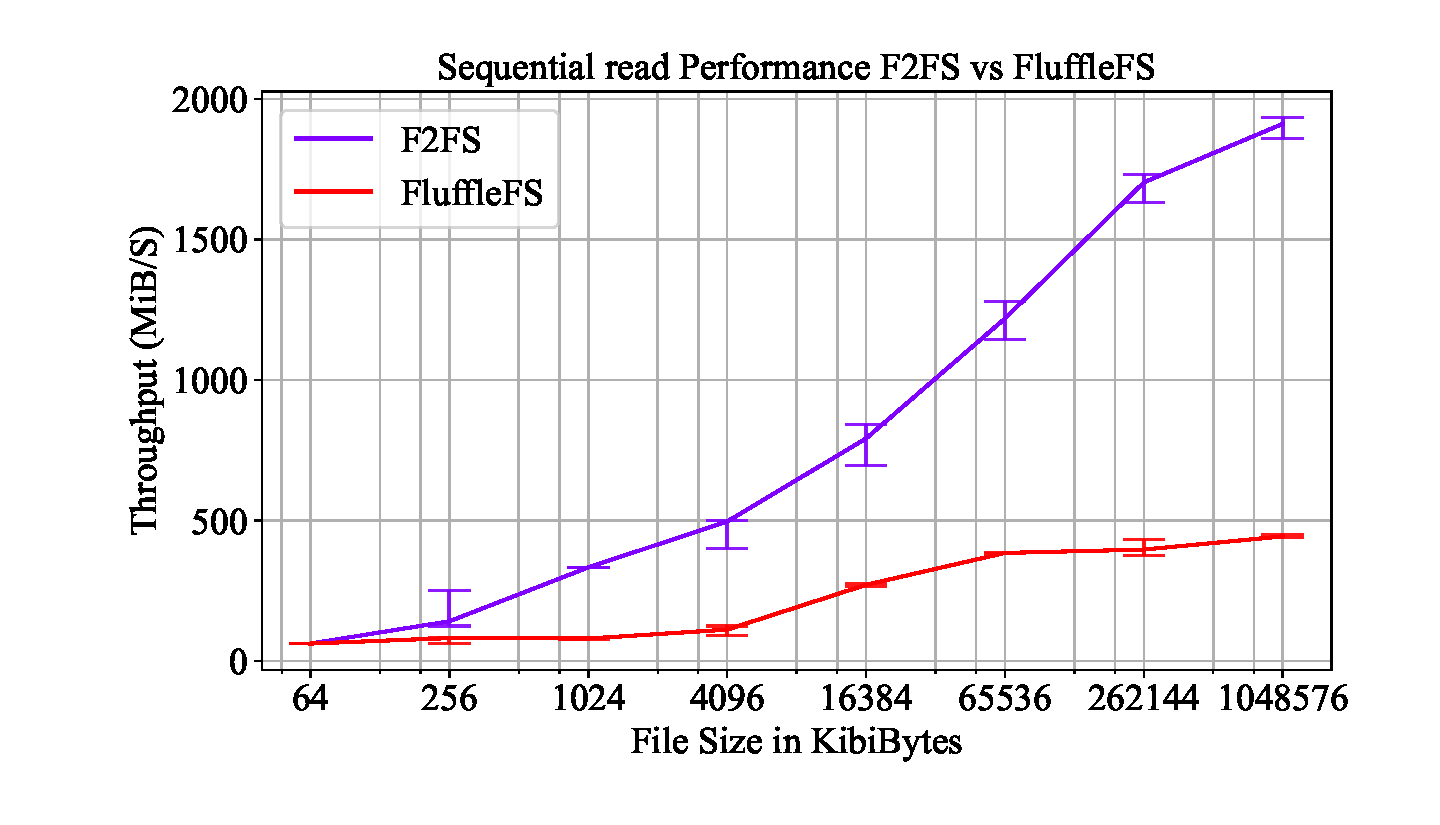
\includegraphics[width=1\textwidth]{resources/images/results-sequential.pdf}
	\caption{Results of sequential read microbenchmark evaluation using a request
        size of 524288 bytes or equal to file size if lesser.}
    % \includesvg[width=0.6\columnwidth]{resources/images/module-dependencies}
    \label{figure:readsequential}
\end{figure}

\begin{figure}[h]
    \centering
	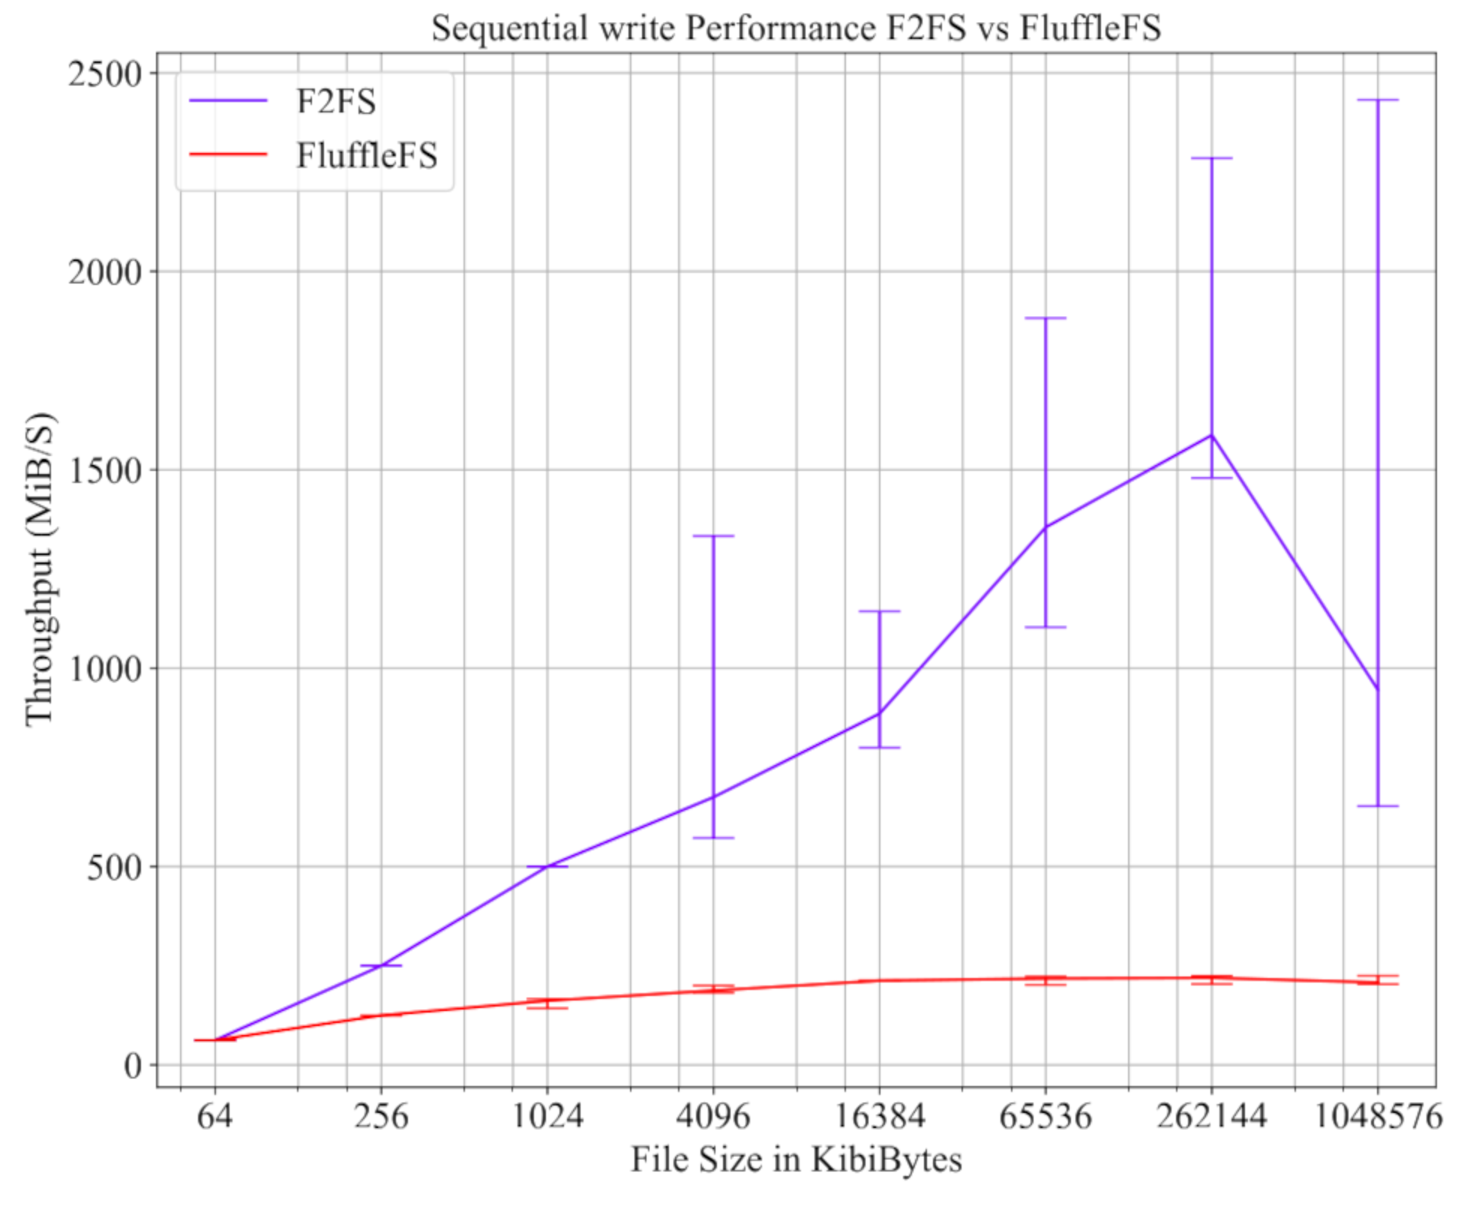
\includegraphics[width=1\textwidth]{resources/images/results-sequential-write.pdf}
	\caption{Results of sequential write microbenchmark evaluation using a request
        size of 524288 bytes or equal to file size if lesser.}
    % \includesvg[width=0.6\columnwidth]{resources/images/module-dependencies}
    \label{figure:writesequential}
\end{figure}

\subsection{Random Results}

Random read and write performance has fastly different results the most notable
is random read performance as shown in figure \ref{figure:readrandom}. Here both
F2FS and FluffleFS reach about 25\% of their previous performance for sequential
reads regarding largest file and request size respectively. Notable is that
the performance of F2FS and FluffleFS is comparable for random reads using a
request size of 4096. Coincidentally, this size is equal to the sector size of
the underlying ZNS device. Furthermore, the performance F2FS achieves for 4096
byte requests maintains roughly equal for lower request sizes. Contrarily,
FluffleFS loses considerable performance for smaller request sizes below
4096 bytes.

Several mechanisms in FluffleFS are likely the cause for this performance
discrepancy. Firstly, FluffleFS submits I/O requests rounded up to the nearest
sector size regardless of how much data it actually needs. Secondly, the
interface between FluffleFS and the NVMe backend perform unnecessary copying of
data. This interface should be updated to use zero-copy instead. Lastly,
FluffleFS allocates and deallocates buffers for each I/O request instead of
reusing previously allocated buffers. Instead FluffleFS should use a memory-pool
only allocating memory during startup and reusing it during the lifetime of the
filesystem. We believe that these are the most likely reason for the
performance difference across small request size random read operation.

\begin{figure}[h]
    \centering
	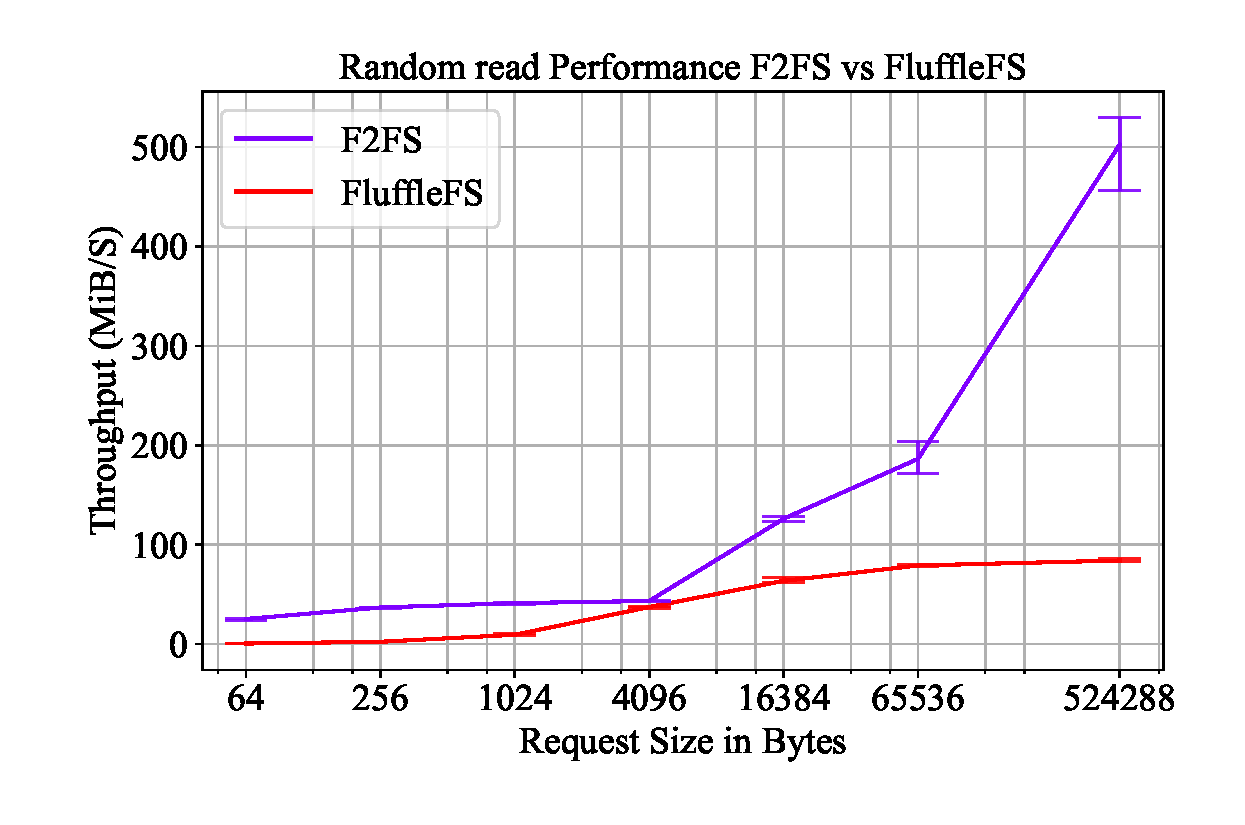
\includegraphics[width=1\textwidth]{resources/images/results-random-read.pdf}
	\caption{Results of random read microbenchmark evaluation using a file size
        of 1GiB}
    % \includesvg[width=0.6\columnwidth]{resources/images/module-dependencies}
    \label{figure:readrandom}
\end{figure}

Regarding random write performance as shown in figure \ref{figure:writerandom}.
Here the performance of FluffleFS is roughly equal to the sequential write
performance. However, F2FS instead has substantially different performance
results. Our first observation is the the random write performance for F2FS is
much higher and more stable with severely smaller difference between the minimum
and maximum. In addition, the mean write performance of F2FS is significantly
higher especially for larger file and request sizes. Most notably is for the
largest results in the sequential and random write benchmarks both file and
request size are identical. Still, the performance difference is substantial and
can only be caused by writing the file sequentially or in random order.

By analysing source code we have determined that F2FS is capable of utilizing
page cache for submitted writes as well as merging incoming I/O requests, writes
and calls to \textit{bio\_put}. Moreover, \textit{bio\_put} is the Linux kernel
block interface and can potentially be used in an asynchronous manner. Given the
large variance observed in write behavior it is likely that write calls complete
before the actual data is flushed to the drive. To investigate how substantially
this write caching influences performance the microbenchmarks can be rerun
using the \textit{O\_DIRECT} and \textit{O\_SYNC} flags upon calling
\textit{open}. Additionally, should the use of these flags proof unsuccessful
the memory contention can be artificially increased by severely limiting the
amount of allocated RAM in virtual machines.

\begin{figure}[h]
    \centering
	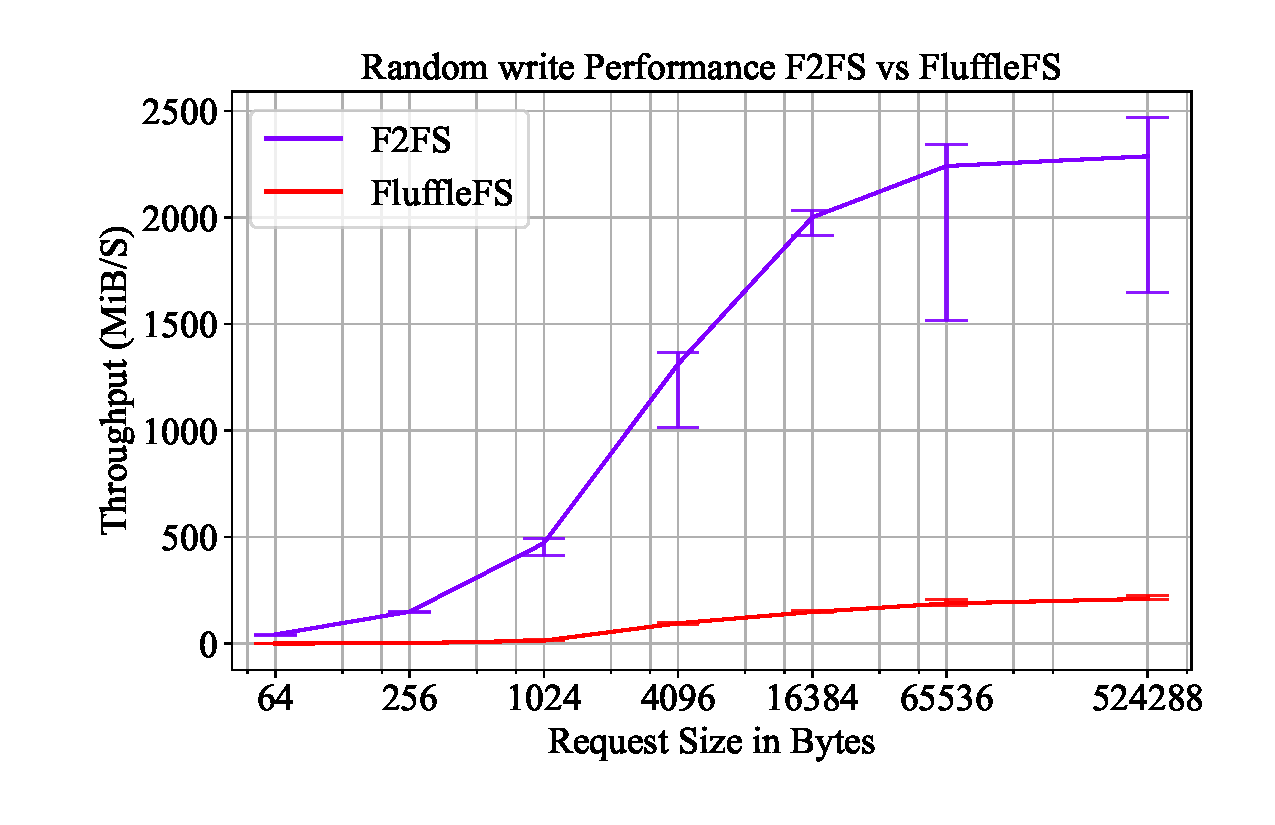
\includegraphics[width=1\textwidth]{resources/images/results-random-write.pdf}
	\caption{Results of random write microbenchmark evaluation using a file size
        of 1GiB}
    % \includesvg[width=0.6\columnwidth]{resources/images/module-dependencies}
    \label{figure:writerandom}
\end{figure}

\subsection{Regular Access Results Discussion}

Similar to sequential reads and writes there is a substantial performance
difference between F2FS and FluffleFS for random reads and writes. Overall the
maximum performance of FluffleFS is considerably low when compared to F2FS. We
have already described three notable differences that might cause such a
performance discrepancy. However, we believe several additional reasons are
further causes of this difference.

Firstly, FUSE based filesystems have to perform additional context switching
between kernel and userspace. A process that has become significantly more
computational intensive due to recently discovered hardware vulnerabilities.
Previous work has shown that between kernel and FUSE based filesystems there can
be a non-negligible performance degradation \cite{Vangoor2017ToFO}. This
degradation was around 83\% in specific workloads with an accompanying increase
in CPU usage of 31\%. However, the minimal performance degradation observed was
just around 5\%.

Secondly, for our specific application the use of inode and data caches as
supported by FUSE had to be explicitly disabled. Otherwise any recent regular
request would influence the return data of an offloaded request if going to the
same region of the same file. It is likely that these inode and data caches are
handled inside the Linux kernel and not by the userspace library of FUSE. 
In the future FluffleFS can likely support inode and data caches by requiring
users to call \textit{open} on offloaded files with the \textit{O\_DIRECT}
flag. However, for our current prototype we have chosen not to investigate this
as this requirement would pose additional barrier to entree.

Third. FluffleFS only submits a single I/O request to the drive moving 4096
bytes per request. This is a very limited method of interacting with the drive
that is likely done substantially differently in F2FS. Not only the performance
differences are evidence that suggests this but explicit management of hot
and cold zones for separate data placement further back this claim.
Additionally, during experimental evaluation the \textit{mq-deadline} I/O
scheduler had to be enabled for the ZNS device to prevent F2FS write errors.
This Linux I/O scheduler serializes outstanding write operations which prevents
the requests inside a ZNS append operation from being reordered. Errors
without the \textit{mq-deadline} scheduler is clear evidence that F2FS submits
multiple I/O requests concurrently.

\subsection{Kernel Passthrough Results}

Our final set of microbenchmarks compare the performance overhead from
offloading to regular access. In addition, we establish the performance impact
on kernels by concurrent regular access. These results are shown in figure
\ref{figure:passthroughresults}. Here we clearly see that the performance
for small file sizes is near identical but starts to diverge more and more
as file size increases. Intuitively we would expect no performance difference
beyond the request size of just 524288 bytes, however, clearly this is not the
case. Most notable is the sudden drop in performance for passthrough beyond
256MiB files. While a similar drop is is observed in the sequential write
performance of F2FS no probable cause is known.

\begin{figure}[h]
    \centering
	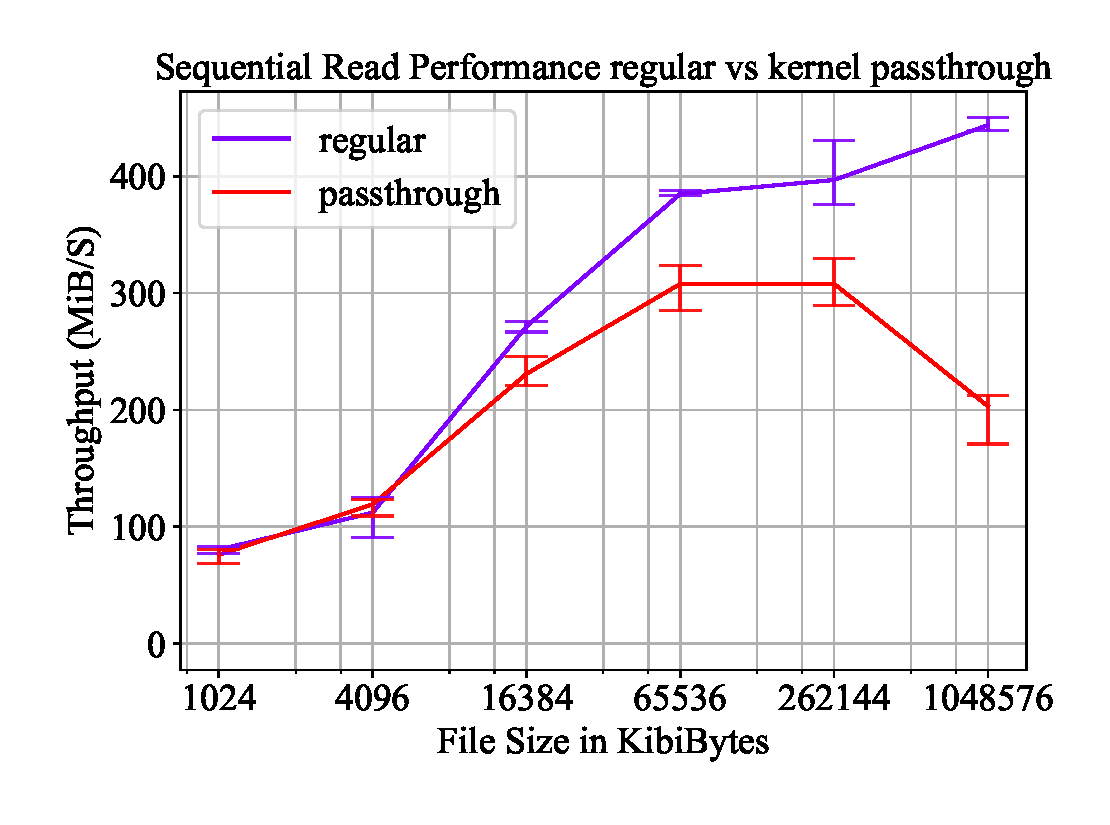
\includegraphics[width=1\textwidth]{resources/images/results-passthrough.pdf}
	\caption{Results Sequential Passthrough}
    % \includesvg[width=0.6\columnwidth]{resources/images/module-dependencies}
    \label{figure:passthroughresults}
\end{figure}

\subsection{Concurrent Access Results}

Our final microbenchmark result is shown in figure
\ref{figure:concurrentpassthrough}. In this figure Dotted lines indicate
baselines from the previous microbenchmark. Furthermore, the red to yellow line
indicates passthrough kernel performance. Contrarily, the blue to cyan line is
used for regular performance. Finally, darker colors represent increasing
numbers of concurrent write jobs scaling from one to four.

From the results shown we can see that both regular and kernel passthrough
performance is still impacted significantly from concurrent write jobs.
However, kernel passthrough has better performance for most file sizes compared
to regular access. These results still show that the concurrent regular and
offloaded access to the same file is able to provide performance benefits.
Unfortunately, we can not conclude that this concurrent performance is entirely
undisturbed. Likely several of the already proposed changes such as submitting
multiple I/O requests concurrently are able to improve concurrent performance
further.

\begin{figure}[h]
    \centering
	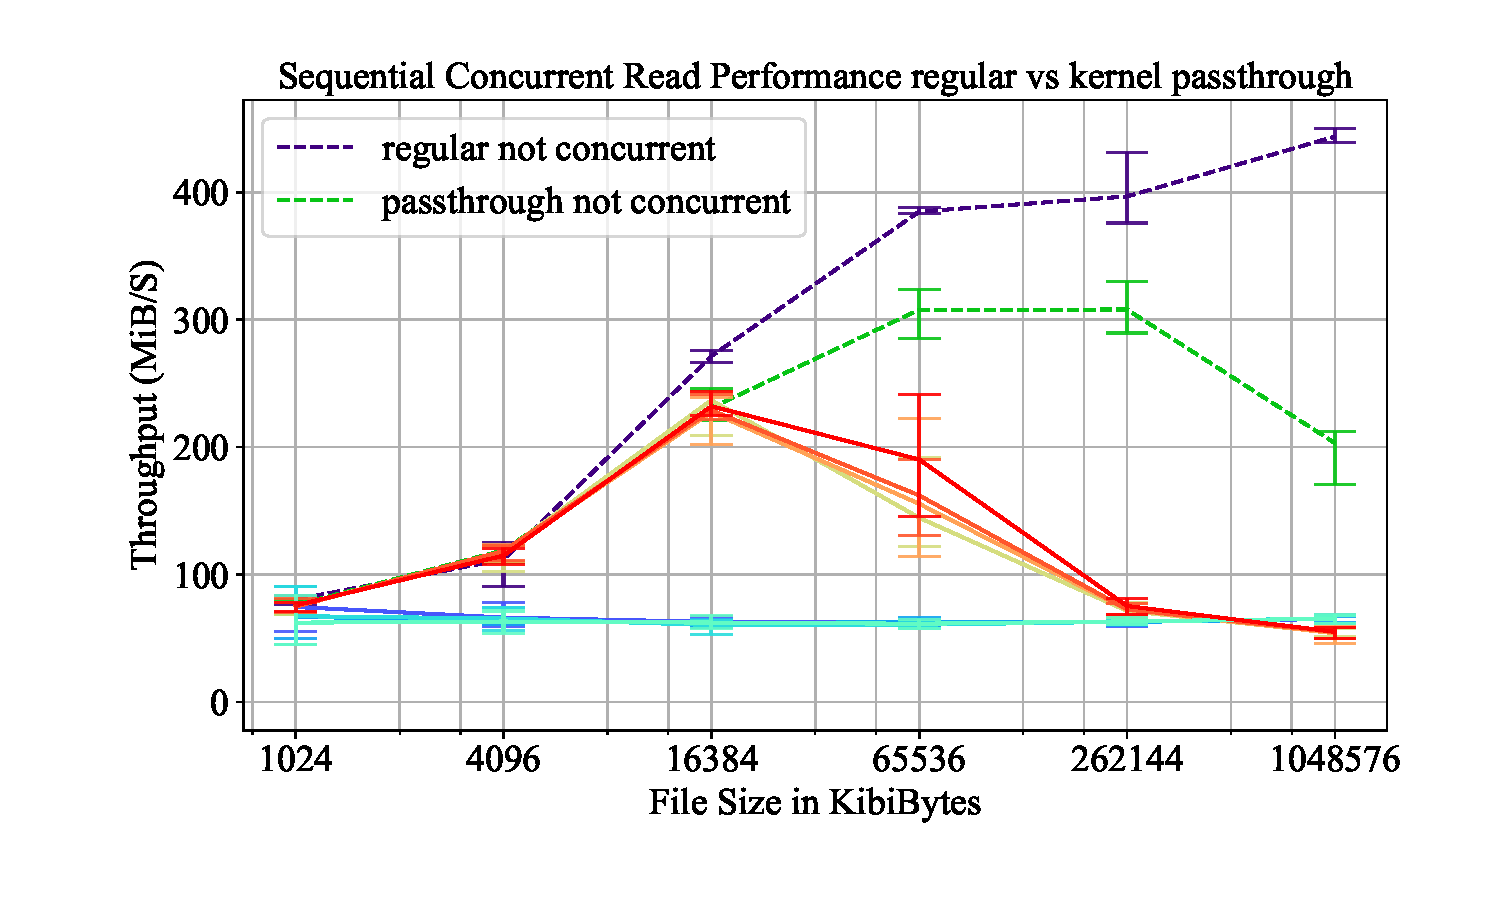
\includegraphics[width=1\textwidth]{resources/images/results-concurrent-read.pdf}
	\caption{Results Concurrent Passthrough.}
    % \includesvg[width=0.6\columnwidth]{resources/images/module-dependencies}
    \label{figure:concurrentpassthrough}
\end{figure}

From these microbenchmarks it is clear that the performance of FluffleFS is
on average significantly lower then top of the line flash optimized filesystem
such as F2FS. However, under a few circumstances both filesystems
performed on par. Given the design requirements and goals of this work this
result is to be expected.

To further improve the performance of this prototype many possible avenues have
been discussed. These are reiterated briefly here. First, I/O requests to
underlying drives  should not be rounded to upper sector size. Second, zero-copy
should be used across interface to reduce data movement. Third, a memory-pool
should be implemented to prevent allocation and de-allocation of memory across
operations. Fourth, inode and data cache functionality should be re-enabled by
requiring the use of the \textit{O\_DIRECT} flag during calls to \textit{open}
when offloading. Fifth, the NVMe backend should be updated to allow multiple
concurrent requests to be submitted to the underlying drive. Finally, the
size of buffers should be increased to allow to move more than 4096 bytes in a
single request.

\section{Shannon Entropy}

In the last results we demonstrate that applications can reduce host CPU load
as well as reduce data movement between the device and host. As discussed the
computation of shannon entropy has been chosen for this.

To evaluate this to implementations to compute shannon entropy are designed.
One written entirely in Python while the other uses Python to combine the
data from individually submitted kernels. Functionality to recombine data from
submitted kernels is necessary as the maximum size of a single I/O request is
524288 bytes (512KiB). For each 512KiB read from the drive only
$256 * 4=1024$ bytes are returned to the host. This constitutes a data reduction
of 1024 times (99.90\%) for this particular application.

In the next two figures the total computation (wall) time of these two
implementations is evaluated using bar graphs. The left hand bar graphs will show
the results for the Python implementation while the right show the offloaded
performance. The total computation time is divided into three categories being
time spent in userspace (user), time spent in kernelspace (sys) and time spent
waiting (wait). Notably, during the time spent in wait the kernel can assign
other processes to run instead reducing CPU host load. Finally, as before the
error bars indicate the minimum and maximum observed difference across all 30
measurements. The results are shown in figures \ref{figure:shannonlow} and
\ref{figure:shannonhigh} for smaller and larger file sizes respectively. Please
Note that the vertical axis between both figures have substantially different
scales.

\begin{figure}[h]
    \centering
	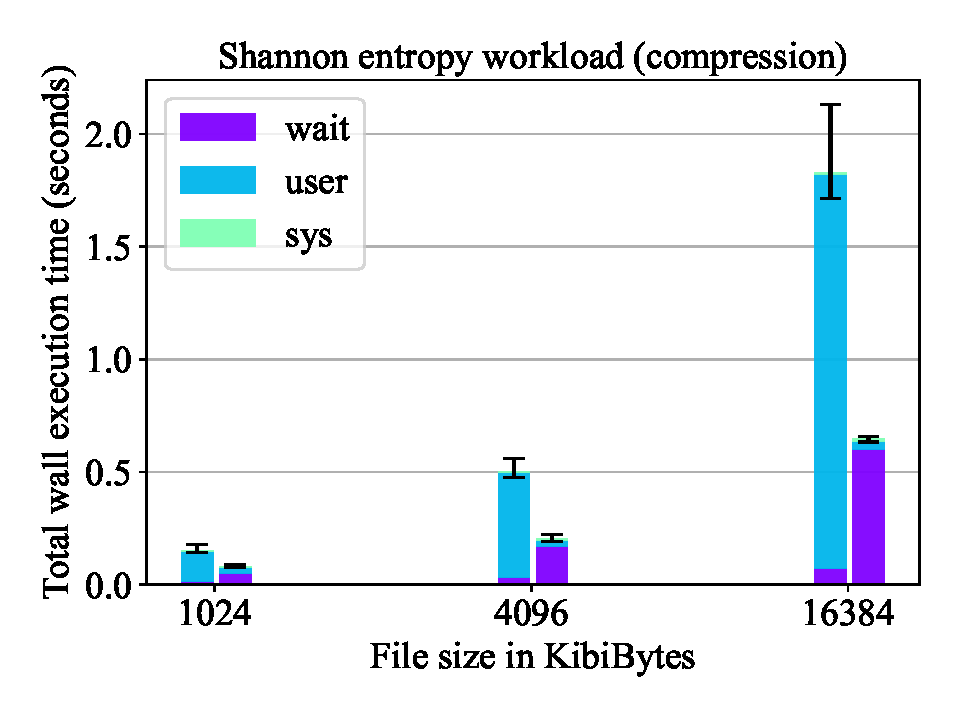
\includegraphics[width=1\textwidth]{resources/images/results-shannon-lower.pdf}
	\caption{Wall time across different contexts for larger file sizes}
    % \includesvg[width=0.6\columnwidth]{resources/images/module-dependencies}
    \label{figure:shannonlow}
\end{figure}

\begin{figure}[h]
    \centering
	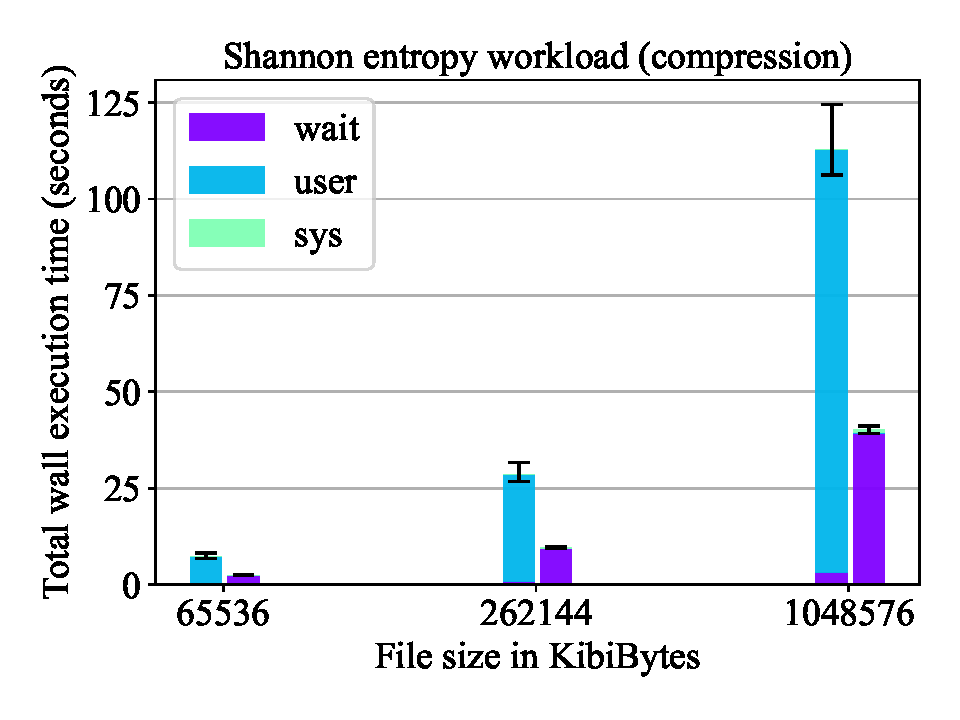
\includegraphics[width=1\textwidth]{resources/images/results-shannon-upper.pdf}
	\caption{Results Sequential Passthrough}
    % \includesvg[width=0.6\columnwidth]{resources/images/module-dependencies}
    \label{figure:shannonhigh}
\end{figure}

Across all these results unanimously our kernel offloaded implementation
is faster compared to our Python implementation. While this not the main goal of
this experiment it is good to see that eBPF \& uBPF can achieve good
performance when using JiT compilation. However, it should be noted that
a fairer comparison would have evaluated a C or C++ implementation against our
offloaded kernel.

Lower execution time inherently reduces the host CPU load. However, this is not
the main observation from these results. Far more important is how almost the
entire execution time of the offloaded application is spent in wait state.
Meaning, that the host CPU is free to perform other tasks while waiting from the
results of the CSx.

Together these results demonstrate that a hybrid filesystem supporting
concurrent regular and offloaded access is able to reduce data movement between
host and device as well as reduce host CPU load in asynchronous applications.

% \subsection{Normalization}

% The compute capabilities of embedded devices such as those that will
% be found on NVMe SSDs and future CSxs is significantly lower compared to the
% host CPU. Will this might change in the future we would have liked to normalize
% our results by differentiating the compute capabilities between the host and
% a commonly found embedded device. Unfortanetely, no vendor releases information
% about the compute capabilities of their NVMe controllers, at least without a
% \textit{Non-Disclosure Argeement} (NDA). Instead we turn to commercially
% available CSxs such as the NGD newport utlizing available literature
% \cite{10.1145/3415580} to estimate the performance of compute cores.

% From this work it can be shown that a NGD newport device contains four ARM A53
% cores that achieve 2.3 DMIPS/MHz. The operating frequency of these cores must be
% between 0.957 and 2.65 GHz. The Dmips performance indication is evaluated using
% a dhrystone benchmark that does not use floating point arithmatic. This is the
% most relavent performance metric available as the computation of shannon entropy
% does not use floating point arithmatic either. Furthermore, the floating point
% capabilities of eBPF are very limited requiring the manual implementation of
% fixed point arithmatic to be performed at all. However, the use of MIPS as 
% performance metric is highly debated as it often is a poor indicator.
% Altneratively, llvm-mca \cite{llvm-mca} can be used to more accurately model the
% number of CPU cycles the kernel would take on each architure. Unfortunately,
% this could not be performed for this normalization due to time constraints.

% Dhrystone 2 using register variables       42381094.2 lps   (10.0 s, 7 samples)

% ---------------------------------------------------------------------------
% ----------------------- end of thesis sub-document ------------------------
% ---------------------------------------------------------------------------